
% to choose your degree
% please un-comment just one of the following
\documentclass[bsc,frontabs,twoside,singlespacing,parskip,deptreport]{infthesis}     % for BSc, BEng etc.
% \documentclass[minf,frontabs,twoside,singlespacing,parskip,deptreport]{infthesis}  % for MInf


\usepackage{graphicx}
\begin{document}

\title{Implementing an online open-source prediction market framework}

\author{Yordan Stoyanov}

% to choose your course
% please un-comment just one of the following
%\course{Artificial Intelligence and Computer Science}
%\course{Artificial Intelligence and Software Engineering}
%\course{Artificial Intelligence and Mathematics}
%\course{Artificial Intelligence and Psychology }   
%\course{Artificial Intelligence with Psychology }   
%\course{Linguistics and Artificial Intelligence}    
%\course{Computer Science}
\course{Software Engineering}
%\course{Computer Science and Electronics}    
%\course{Electronics and Software Engineering}    
%\course{Computer Science and Management Science}    
%\course{Computer Science and Mathematics}
%\course{Computer Science and Physics}  
%\course{Computer Science and Statistics}    

% to choose your report type
% please un-comment just one of the following
%\project{Undergraduate Dissertation} % CS&E, E&SE, AI&L
%\project{Undergraduate Thesis} % AI%Psy
\project{4th Year Project Report}

\date{\today}

\abstract{
Model aggregation, markets, prediction markets. 

My market
}

\maketitle

\section*{Acknowledgements}
You guys have been a great inspiration!

\tableofcontents

%\pagenumbering{arabic}


\chapter{Introduction}

Information has been traded extensively in one way or another since the dawn of man. Intuitively this is true, but is even truer in recent years with advances such as the information economy and big data transforming the way we think about data and the knowledge it carries \cite{mcgee_managing_1993}; at the same time it has never been harder to quantify its value. 


The problem of efficiently combining information coming from different sources in order to form a rational belief is largely an unsolved issue in Bayesian philosophy \cite{greene_collective_2010}. It manifests in the domain of machine learning as the problem of belief aggregation which is the use of a number of existing machine learning algorithms in order to achieve better predictive performance. It is usually addressed using a number of diferent approaches. In practice though existing algorithms such as boosting, or expert products or mixtures are not as flexible as they introduce various constraints. and are rarely useful out-of-the-box. This in turn means that often result in complicated, task-specific solutions.

	If we take a look at ordinary commodity trading though it is apparent that the existence of a market where agents can exchange goods using a common currency provides a meaningful way to determine the prices of the traded goods. The simplest form of such a market needs not be active with regard to the traded goods and is nothing more than the market squares that have existed in towns for ages. A more recent example are stock markets which nqkaksi agree on the price of stuff. By following the market's trading activity we could then obtain a good idea of the value associated with each of the traded goods in the market. 

	A prediction market is a special kind of a market which allows agents to trade on and share their information of a future event with the public. This is achieved by designing a market where the trading goods are akin to shares corresponding to each of the possible outcomes of the events of interest. Each share promises a fixed payment in the future to its holder if and only if the outcome associated with it happens to be the event's actual result. This future point is usually fixed at the start of each challenge, and is necessarily after the result of the event has been observed by the public. Disregarding arbitrage opportunities we can then treat the goods' prices as a probability distribution over the outcome space. 
	
	
	For example a binary event is either going to happen or not. If the price of purchasing one of each share is less than the reward promised by each of the shares there's an opportunity for making {\em risk-free} trades.  we   with regard to the trades we could then be This setup incentivises players whose beliefs differ from those of the market to act on the difference in prices. Consider a rational agent whose beliefs differ to the currently established market price. Such an agent is incentivised to trade on the observed difference. By doing so he informs the market of his position and helps establish an equlibrium price. 

	My project deals with the implementation of a flexible online prediction market framework. In contrast to existing solutions  though it is mostly intended as a clean and extensible framework to be used as a base for further efforts. To this end the software offers a concise, well-tested and documented prediction market core with a modular architecture which allows for the creation and experimental comparsion of different pricing algorithms. Being an online platform it has a full-featured though fairly unsophisticated user interface, but also includes a comprehensive user-facing API which permits and actually encourages algorithmic trading. Additionally the market can host entirely automated competitions which can be used as an addition to supervised classifiers to improve predictive performance. 

	A more advanced goal is the creation of a market where players are encouraged to build automated trading algorithms that predict and bet on the outcome of a (family of) events.  in a way turning it into a crowdsourced machine learning competition. Such an approach towards machine learning problems is not entirely new, prominent examples being the {\em Netflix prize} challenge which was held as early as 2006, and the {\em Kaggle} online platform which hosts such competitions. A major distinction is that while existing approaches operate in a {\em winner takess all} manner

\chapter{Related Work}

	In this section I will go over the existing approaches to model aggregation, prediction markets, and how they connect to each other. I will then review some case studies of prediction markets at work. Finally I will have a look at the existing solutions that could be used as a base for my project. 

\section{Model Aggregation}
	In machine learning the problem of model or belief aggregation deals with the creation of meta-algorithms that use a set of existing supervised classifiers for a task in order to obtain better predicitve performance in comparison to any of the constituent algorithms alone. 

\section{Machine Learning Markets}
% mention Amos' research

\section{Existing Software}
% 
	My search for software started first and foremost with  investigation of the open-source solutions which I could use as a starting point for my project. 
	When looking at the existing software dealing with prediction markets of immediate interest are the open source platforms which could be used as a base of the project. I also looked 
% briefly say we need (open source, extendable, easy to learn and use) framework
% go thru zocalo, (drupal addon), 

\subsection{Open source}
	My search for open-source projects yielded the following results:

\begin{itemize}
\item {\tt Zocalo}

	Zocalo is an MIT-licensed prediction market written in Java using Java Server Pages (JSP) and Hibernate. It is probably the most prominent of the listed examples having been used in a number of research projects already. It allows the creation of both {\em order book} and {\em market maker}-based markets of single discrete variables. Although it supports real-time updates via AJAX the user interface is fairly simple with the HTML being stitched on the fly using Java. This and the fact that the codebase is already large and tightly coupled means it may be difficult to extend or modify existing parts of the software. There is also no public market API and writing one in addition to supporting multinomial markets could prove hard due to the reasons listed above. 

\item {\tt ideafutures } \footnote{http://ideafutures.sourceforge.net/}
	{\tt Ideafutures} seems to be one of the first online prediction markets in existence dating as far back as 1995. It has been featured in a number of publications (cite). Although it only supports markets of single boolean variables. 

Although it is still used by the aforementioned market, development on the software seems to have stopped since 2005. It is written in Perl and uses BerkeleyDB.  but is also inactive since 2005, although the not-for-profit closed-source prediction market Foresight Exchange seems to use it with success. 

\item {\tt Open Prediction Markets} 
	Drupal is a modular, open-source content management system written in PHP. {\tt Open Prediction Markets} is a Drupal module which implements prediction market functionality. 
\end{itemize}

% disuss why I didn't choose any of those. 

\subsection{ Commercial }
	Of note is also the presence of a number of (closed-source) commercial prediction market implementations that could be used as [a point of reference] in terms of features and flexibility. Due to futures markets being regulated in many parts of the world, most of the markets I looked at use alternative currencies such as Bitcoin. 
 dealing in bitcoin such as bitbet.us (implementing a parimutuel payout strategy), predictio.us (an order-book market), and fairlay.com (market maker-based). The last few examples also present different options for visualising the activity and structure of the markets such as price histograms, market depth graphs, and interactive UI.
\begin{itemize}

\item {\tt hm? }

\item {\tt bitbet.us}
	BitBet is a website where participants can use Bitcoin to play in parimutuel markets of binary outcomes. Thanks to the simple market mechanism its interface and betting process are fairly streamlined with intuitive visualisations and registration-free betting using Bitcoin and QR-codes. While it is not strictly a prediction market as it doesn't deal with securities it strikes mostly with its minimalistic and clean user experience. 

\item {\tt Predictio.us}
	Similarly to the previous example this website uses Bitcoin and supports only markets of binary variables. It is also a proper prediction market albeit entirely passive: there is no market maker and an order book is used instead. This limits the usability of the market 

	It also has a more involved 

to provide prediction markets for a number of topics ranging from sports to science. 
\item {\tt Fairlay}	
	
% \item {\tt Inkling}	Although not a prediction market per se, {\tt Inkling} offers a prediction market infrastructure as a service to businesses and organizations. 

\end{itemize}
\chapter{Definitions}
% TODO: is this even needed?
% Define markets, prediction markets. Detail how we use them to aggregate beliefs. 

\section{Market}
	Markets provide a common ground for the exchange of goods between different agents. Basic markets are netural towards both the participants and the goods being traded and do not have the concept of currency which is seen as another good instead. Each of the agents has an associated {\em position} in each of the goods being traded in the market which is simply the amount of the good they currently possess. In general there is no restriction on the value of the agent's position and we will distinguish between {\em long positions} where the agent has a positive holding, and {\em short positions} where the agent has a negative amount of the good. 

	A basic model of such a market is the {\em order book} which records and matches the bids and offers placed by participating agents. Note that there is an inherent degree of freedom when implementing the matching process: arbitrage opportunities must be dealt with care if the market is to be strictly neutral, and the same goes for partially completing orders (since rarely, if ever both the price and the quantity match). 

\section{Prediction Market}
	Prediction markets are a type of market with an agreed currency where each of the remaining goods is tied to exactly one of the possible outcomes of a future event. Each good promises a fixed reward (taken to be 1 credit for simplicity) in case the outcome associated with it happens to be the event's actual result, and zero otherwise. Goods can be additionally created by agents for sale, which is equivalent to the agent assuming a short position in the market. 

	Prediction markets have been used in the past in health care (Polgreen et al. 2006), to aid decision-taking in large corporations (Cowgill et al., 2008), and to predict presidential elections (Dudik et al., 2012). Recently prediction markets such as intrade.com were also shown to provide more accurate results on the Scottish referendum as compared to traditional voter polls (Bell, 2014).

\section{Machine Learning Markets}
	Machine learning markets are a fairly recent extension of the idea of prediction markets where the participants are machine learning agents acting according to a given utility or betting function. As such the research in this area is limited

\chapter{Project Scope}
	Here I outline the scope of the project in terms of the major milestones that I accomplished. 



\section{Accomplished Goals and Milestones}	

\subsection{Design a simple, expressive prediction market framework}
	% talk about bduf, agile and finance software needs 2 be reliable
	This involves modeling the market-player relations from the market maker’s view in a structured and sane fashion. 

Allow the placing of orders (bets) using a human-facing web interface and market management using simple Python commands or (optionally) a web admin interface. It should be possible to track and advance challenges (representing the true results for the current iteration) in a market, and raise events to announce the arrival of orders and challenge progression to the corresponding market maker modules. 

\subsection{Write a modular market maker model}

Market makers control the exchange of goods and their prices and are thus vital to the predictive performance in the resulting market. I will look in detail at algorithms for price formation in prediction markets including scoring-rule based ones, parimutuel betting schemes, but also more involved models which establish clearer connection between the actions of traders and their underlying beliefs. observed prices and the underlying probability of outcomes such as the ones described by Barbu and Lay 

\subsection{Write a simple yet sufficient user inteface}
	The user interface is arguably one of the more important aspects of the software when it comes to [players staying and coming to the market]. It should offer basic functionality such as following and playing in a market, but also present the important bits in an informative way. 
	

\subsection{Allow programmatic access}
	The ability to use an API in order to manage and interact with the prediction markets would allow the execution of experiments where some or all of the participants are automated. In light of recent studies (see Chapter 4) such a tool could be used to experimentally establish equivalences between particular market setups and machine learning algorithms. As this feature could be used by participating humans, it could additionally become a framework 

	An important consequence of this feature will be the possibility to run prediction markets where players are encouraged to write their own machine learning algorithms in order to beat the problem at hand. While there are existing platforms that deal with the same problem of designing a machine learning classifiers using crowdsourcing (e.g. {\tt kaggle.com}), they do so in an inherently competitive (and thus non-collaborative) winner-takes-all model. In contrast prediction or machine learning markets allow the elicitation of beliefs based on the performance of {\em all} of the participating agents. 

\section{Future Work}

\subsection{Implement an intuitive and dynamic UI}
	When I approached the project I had close to zero experience with any of HTML, JavaScript or CSS. This meant I had to start off more slowly and spend a sizeable amount of time getting the static structure of the interface done. Although I wished to additionally 

\subsection{Event/Variable Composition}

\chapter{Implementation}

\section{Design}
	This chapter details the design decisions taken while building the project. I first talk briefly about the technologies I decided to use and why I started from scratch. I 

	This chapter outlines the major architectural decisions taken before and during the implementation of the project. I first talk briefly about the reasons for starting a new project instead of extending an existing one. I then continue by examining existing software stacks in terms of how suitable the language and libraries are for the task at hand. Finally I outline the major architectural components of the completed project and the ways they interact with each other. 

	When approaching the project one of my main goals was to build a software which could be both used and extended easily. On the other hand the specific nature of the project - financial prediction markets - means that it should be easy to both understand and verify the correctness of the code. These two goals are inherently clashing: 
With this in mind I explored the following choices of programming platforms:

\begin{itemize}
\item Python

Python is a popular dynamic language supporting a number of programming paradigms. In addition to its comprehensive standard library there is a variety of available packages that cover a wide range of functionality notably in terms of web development. Django\footnote{https://www.Djangoproject.com/} is a popular full-stack framework which supports a number of database back-ends and emphasises modularity and readability. There are also a number of packages with a minimalistic approach such as Flask and Pyramid which allow for custom tailoring of much of the underlying processes. 

On the other hand the dynamic nature of Python can quickly become a burden when dealing with bigger projects. Why?

\item Java

While it is a popular choice for commercial software thanks to its wide platform support and interoperability, writing web applications in Java has its drawbacks in comparison to other languages better suited to the task. Since it is a static, compiled language it is easier to verify some aspects of a program's correctness as compared to dynamic languages, but that comes at the cost of not being able to quickly observe the effects of code changes as is possible with the latter. In addition Java applications tend to add a significant architectural overhead resulting in a clunkier code. 

\item .NET

	Although not as widely used as the previous two examples the .NET Framework would have been my choice of platform in the beginning. It offers a full MVC framework - Asp.NET -  similarly to the previous two examples but also includes languages that together could outperform either. For example the code for the market structure could be written in C\# (which while highly similar to Java is also arguably more concise and expressive) while advanced market makers can be implemented in the functional F\# language instead. 

	A major drawback of the platform is that even though it is popular amongst Windows users and select businesses, it lacks a strong open-source community and infrastructure. Although the latter has been remedied as of recently by the release of much of the .NET toolchain as open-source projects on Github, that was not the case when I was starting the project. 

\end{itemize}

	I finally decided to use Python mainly due to its ubiquitous use and the availablity of packages, discussions and general presence on the Internet. The latter proved invaluable since whenever I stumbled across difficulty while writing the actual implementation, I found that looking up discussions on similar problems on sites such as {\tt stackoverflow} was of great help. Although that's not necessarily a plus and may reflect a weakness in the language or its philosophy, I managed to overcome most, if not all, the problems I was faced with. 

	My biggest issue with the language was the fact that it is dynamic. While such languages make fast prototyping of software much more straightforward, they are quickly overshadowed by their static counterparts when it comes to dealing with bigger applications involving a fairly stable design and implementation. For example even though I used the Visual Studio IDE which has a great syntax highlighter and code completion features, it would constantly lose the type information of variables due to intricacies inherent in the framework and the language. In the end I felt like I spent a lot of time manually verifying and ``type-checking" my programs, and ultimately debugging them: a problem that would be irrelevant in the context of a static language. 
	
	For a web framework I chose Django due to the similar concerns: while there were some simpler alternatives, in terms of both architecture and capabilities, I decided I would rather have access to all the benefits of Django - 

it tries to follow an idiomatic (or {\tt pythonic}) syntax and similarly has the largest user-base and amount of tutorials written for it. Although one of the simpler 
	These two choices also offered the widest range of useful modules to assist with the various components I would need in the final software. This includes small stand-alone packages such as {\tt django-graphviz} which  the visualising the database models in the program  

While I still believe this is a good stack to use for the task at hand, it imminently lacks some of the features I’d need like framework support for real-time applications. On the other hand there is at least one third-party package dealing with this so implementing it may still be straightforward. 
	

	
	During the first month of the project I worked on writing the common market structures as well as the web views for players to register and interact with them. A full class diagram along with a brief description of the application’s architecture is shown in Figure 1. Creation and management of markets, their datasets and events can be currently done via a web interface (using the built-in django-admin package), by Python programs running on the same machine as the markets, or from a RESTful API.
The whole pricing and order handling logic comprising the market makers is written as modules controlled by the core ml-markets application. Each module provides price quotes, handles orders, and distributes winnings to players. This allows each market to specify the type of pricing engine to use but also helps for running markets under different scenarios which will come handy when evaluating their performance.  

\section{Market Structure}
% talk about the specific design decisions when making the markets
In this section I talk of the internal structure of the markets in the final software. I introduce the main components of a prediction market from a programming viewpoint and the ways they interact with each other. I talk about some of the design decisions I was faced with while writing the code and the took while implementing the core market structure

\subsection{Models}
    Models are the main building block of Django's ORM approach. Written in Python much like normal classes they are used by the framework to recognise and automatically apply changes to the underlying database back-end. Models represent a fairly lightweight layer over traditional SQL constructs as their structure is necessarily flat and explicit relations such as keys and field multiplicity should be specified. Nonetheless it achieves its purpose of eliminating code duplication and database overhead in a fairly elegant, {\em pythonic} way. I found the advanced, if at times complex, tools for querying and updating the database were expressive enough for the purposes of the project. 

    The purpose of a prediction market is to model the probability space defined over one or a number of related variables or events such as the performance of public companies or sports teams. 
    
    
    At the core of the software stands the {\tt Market} model which is the basic representation of a prediction market. As part of its basic functionality every prediction market should keep track of the active players, process incoming orders in terms of the traded goods, and finally resolve shares (or goods) to rewards at the end of its lifetime. Since we are interested in modeling discrete, multinomial outcome spaces we associate each {\tt Market} with the variables or {\tt Events} specific to it. While in traditional prediction markets model we are often interested in modeling a specific instance of a problem, in machine learning markets we are necessarily modeling a {\em family} of events instead. Consider for example 
    
     their successful application in machine learning context necessarily involves the consideration of a {\em family} of events . 


\begin{figure}
\centerline{ 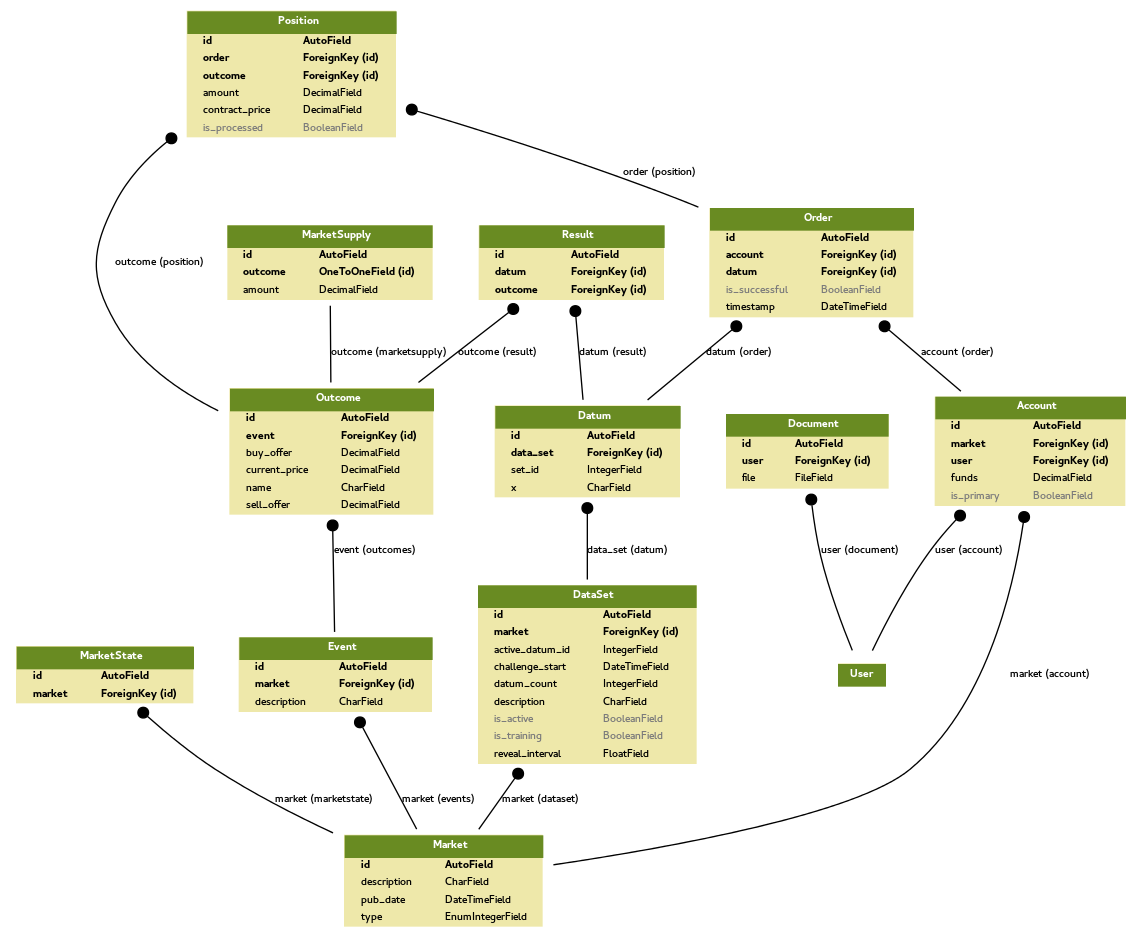
\includegraphics[scale=0.7]{markets_graph.png} }
\label{fig:class_diagram}
\caption{Class diagram of the models comprising the market core. }
\end{figure}

\subsection{Admin Interface}
The admin interface is the place where market operators can create and configure the hosted markets and manage their contents in terms of variables (events) and data sets. 

	Since the framework comes with the built-in {\tt django-admin} module serving this exact purpose, implementing the interface was not as terrifying as I had initially feared. Most common but often tediously repetitive operations - such as creating, editing or deleting objects - were surprisingly easy to implement thanks to the built-in capabilities of the module. On the other hand other less ``popular" features, such as the option to pre-fill a dataset with randomised entries or 

\subsection{API}
	Implementing a remote API was one of the more important features of the project due to two reasons. 
\section{Market Makers}
% talk about the market makers that were or can be implemented. 
	What follows is a brief overview of the pricing algorithms investigated in the scope of the project. As part of my design goals the existing market structure allows for the implementation of a number of different market pricing mechanisms. To 

\subsection{Interface}
	The two basic actions market makers should provide are processing orders and finalising challenges. 
	
\subsection{Order Book}
	
	The “city plaza” market scenario where potential buyers and sellers all place their bids and the matching buy/sell offers are resolved. There is normally more than one way to complete trades where for example an agent sells at a price lower than that of a matching buyer, or an agent wishes to buy a larger quantity than a seller has to offer. Usually the market maker is neutral towards both the goods and their prices, but can also be made active by e.g. resolving arbitrage opportunities in his favor.

	Although they are simple to implement and operate, auctions of this type tend to create thin markets with volatile prices and low liquidity of the assets being traded. We can furthermore use the concept of Nash Equilibria to show that such markets do not incentivize players to share their true beliefs and are thus not well suited for model estimation (Myerson et al. 1983). Consider for example a buyer who values a given good well above its current market price: he or she would have no incentive whatsoever to let others (“the market”) know about their high valuation of the good but will instead seek to make trades at the lower price.
	
\subsection{Parimutuel Betting}
This is the system usually used in gambling on sporting events, or in various lotteries. In it all bets of a type are put together in a pool, and the instantaneous odds are determined by the ratios between the already placed bets. The final winnings are determined by sharing the pool (minus any house cuts) amongst the winning bets. Although easy to implement and operate, such markets do not offer any guarantees on the amount to be won in case of success (i.e. the final odds) since the latter isn’t known until all bets are collected.

\subsection{Market Scoring Rule}
In a market scoring rule (MSR) prediction market agents report a probability estimate r on the outcomes of an event and are rewarded sci(r) when outcome i happens. Proper scoring rules are rules which reward estimates close to the truth the highest and penalise estimates that deviate from it, thus incentivizing players to act according to their true beliefs.

 [TODO: Review] Such scoring rules are typically monotonically increasing, an example being sci(r)=a+bilog(ri) which is the logarithmic market scoring rule (log-MSR; Hanson, 2002). It is a proper scoring rule which quantifies the risk (also known as self-information in information theory) for the market maker at any time and charges participants proportionally to the change in risk their positions incur: players who move the market prediction towards the “true” distribution (or winning outcomes) get rewarded for doing so, while those who degrade the market prediction are penalised.

In general MSR market schemes are more involved than other examples but also allow for greater flexibility in the pricing strategies. 

\section{User Interface}
% mention the static interface, js graphics !!

	Due to my limited abilities in html and javascript the current user interface is fairly simple. Apart from basic features such as (secure) user registration and login it provides price quotes and transaction history for markets. There are a few directions I would like to expand on: for example by including histographs to visualise the prices or the trade volume in a market, by allowing browsing other agents’ portfolios, and making the interface more intuitive as a general. A great case study is presented in “A Combinatorial Prediction Market for the U.S. Elections” by Dudik et. al

\section{Other Tools}

\subsection{django-extensions}
    This package is an MIT-licensed collection of extension tools which ease the process of developing Django apps. Two most useful features I used were the ability to automatically generate {\tt django-admin} templates and GraphViz {\tt dot} files of the models in a package. The latter especially helped me visualise [TODO: Also does what?]


\section{Testing and Documentation}
% documentation at github.io ?!
% issue tracker ?!?!
% wiki too ?!?!?!?
	When it comes to designing and testing an application dealing with any kind of transactions, it is clear that a set of minimum requirements has to be met in terms of consistency and transaction atomicity. Fortunately the high-level nature of the language and the framework make this straightforward. 

	I initially wanted to adopt a test-driven approach towards units tests but doing so proved hard for the first few months of the project. Since it is straightforward to introduce runtime validation or assertions in Python I used that extensively from the start. 
\subsection{Unit Tests}
	During that time I was mainly modeling the market structure and writing code for the front-end. Most of the work was thus of declarative nature and needed little, if any, tests as long as the design was OK. 

	The testing process was not without its quirks related to the framework I used. After I completed the first few tests and proceeded to run them I noted they were all failing in a very specific way: although I could create objects in the test database and manipulate them referentially, accessing them using query selectors inevitably failed. 
	While I was implementing the market makers I could find more test targets in terms of functionality. This allowed me to statically verify some of the assertions made 
While I had trouble creating a comprehensive automated test suite though. I currently have a few simplistic tests (i.e. voting for A in a new market should increase the price for A) but I can’t find obvious targets to include in the suite.
\subsection{Runtime Tests}
    There are a multitude of runtime tests achieving custom validation on top of Django’s existing model validation, but also hard assertions for model invariants. For example the joint asset prices for an outcome space always summing to 1 is enforced throughout the market makers, but there are also explicit checks executed every time prices change.

    While designing the base models I paid extra attention to transaction atomicity: it would be quite inappropriate if funds appeared or vanished while serving requests in a market. Thankfully the framework makes implementing this easy and idiomatic enough so I had no problems accomplishing it using method decorators and with blocks.

\subsection{Documentation}
    As an important part of 
    As an integral part of the development of a maintainable and useful software I decided I needed to have a documentation process which is flexible enough to both generate {\em AutoDoc}-style descriptions   
    
\subsection{Issues}
    As I was using the 
\chapter{Evaluation/Reflection}

\chapter{Conclusion}
	Prediction markets have already been studied for a while. Nonetheless there are 
% its a stepping stone for creating advanced prediction markets. Hopefully not rough. 




% use the following and \cite{} as above if you use BibTeX
% otherwise generate bibtem entries
\bibliographystyle{unsrt}
\bibliography{ixlib}

\end{document}
